%%%%%%%%%%%%%%%%%%%%%%%%%%%%%%%%%%%%%%%%%%%%%%%%%%%%%%%%%%%%%%%%%%%%%%%% 
%%%%%%%%%%%%%%%%%%%%%%%%%%%%%%%%%%%%%%%%%%%%%%%%%%%%%%%%%%%%%%%%%%%%%%%% 
\begin{frame}
  \frametitle{Ouessant : IBM Power8 + Nvidia Pascal P100}
  
  \begin{itemize}
  \item {\bf \textcolor{violet}{\large About ouessant computing platform}}
    \begin{itemize}
    \item online ouessant user guide : \myurl{http://www.idris.fr/media/ouessant/ouessant-user_guide.pdf}
    \item Use material from IBM/NVidia~\footnote{Thanks to Nicolas Tallet and P. Vezolle (IBM)}, gives detail on the platform\\
      See file: \myurl{doc/ouessant/Introduction_ouessant_2017.pdf} in archive
    \item Minimal information about software environment, how to build and run an application, submit a job on machine \texttt{ouessant}\\
      See file: \myurl{doc/ouessant/Ouessant-Application_User_Guide-16-12-1.pdf}
    \item {\bf Examples of job submission scripts:}\\
      \myurl{/pwrlocal/ibmccmpl/share/templates/lsf}\\
      You will need to understand the basics of task affinity on Power architecture (p8aff).\\
      \myhref{https://www.ibm.com/support/knowledgecenter/en/SSWRJV_10.1.0/lsf_admin/affinity_power8_lsf_submit.html}{affinity\_power8\_lsf\_submit.html}
    \end{itemize}
  \end{itemize}
\end{frame}

%%%%%%%%%%%%%%%%%%%%%%%%%%%%%%%%%%%%%%%%%%%%%%%%%%%%%%%%%%%%%%%%%%%%%%%% 
%%%%%%%%%%%%%%%%%%%%%%%%%%%%%%%%%%%%%%%%%%%%%%%%%%%%%%%%%%%%%%%%%%%%%%%% 
\begin{frame}
  \frametitle{Ouessant : IBM Power8 + Nvidia Pascal P100}
  
  \begin{itemize}
  \item {\bf \textcolor{violet}{\large About ouessant computing platform}}
    \begin{itemize}
    \item \textcolor{red}{\bf CPU is IBM Power8} - {\bf see output of lstopo}
    \item \textcolor{darkgreen}{\bf GPU are K80 (on login nodes) and P100 (on compute nodes)}
    \end{itemize}
    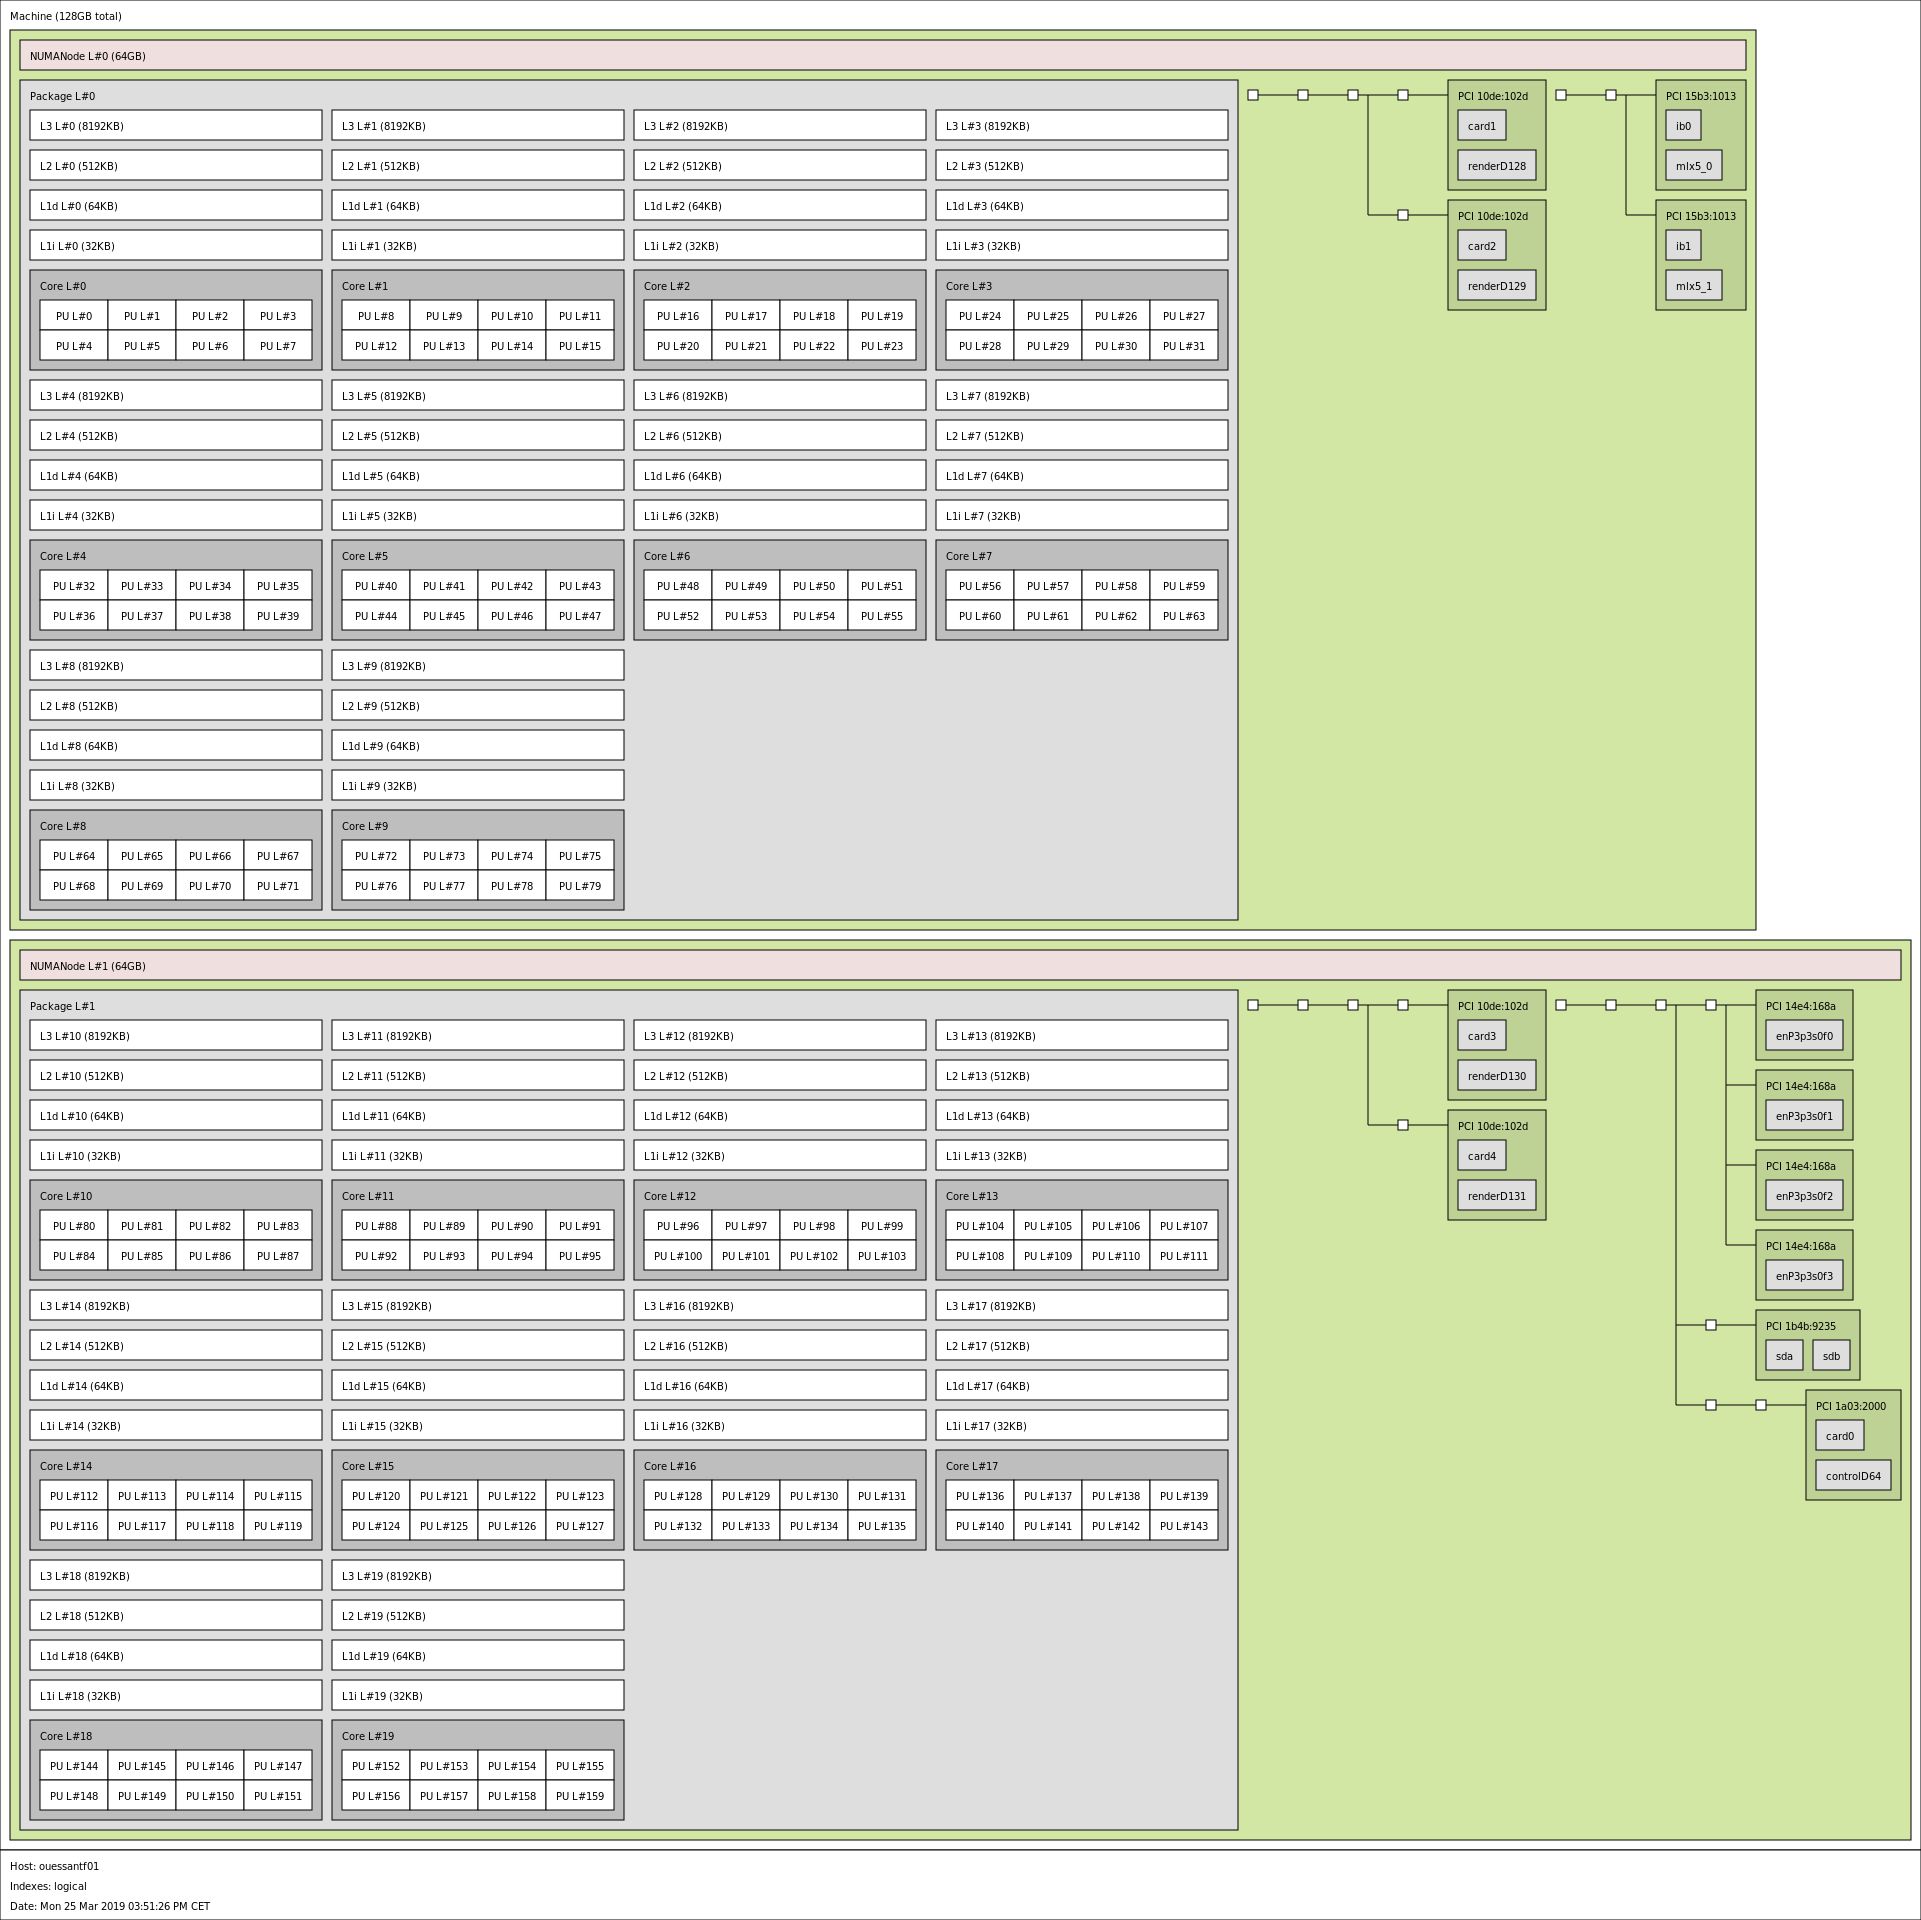
\includegraphics[width=6cm]{images/ouessant_lstopo}
    % on ouessant : lstopo-no-graphics -p ouessant_lstopo.xml
    % on desktop : lstopo -i ouessant_lstopo.xml -l ouessant_lstopo.png
  \end{itemize}

\end{frame}

%%%%%%%%%%%%%%%%%%%%%%%%%%%%%%%%%%%%%%%%%%%%%%%%%%%%%%%%%%%%%%%%%%%%%%%% 
%%%%%%%%%%%%%%%%%%%%%%%%%%%%%%%%%%%%%%%%%%%%%%%%%%%%%%%%%%%%%%%%%%%%%%%% 
\begin{frame}
  \frametitle{Kokkos training material}
  
  \begin{itemize}
  \item {\bf \textcolor{violet}{\large Official Kokkos documentation}}
    \begin{itemize}
    \item {\bf Wiki on github :} \myurl{https://github.com/kokkos/kokkos/wiki}
    \item {\bf Kokkos programming guide} in sources : \myurl{https://github.com/kokkos/kokkos/blob/master/doc/Kokkos_PG.pdf}
    \item {\bf Doxygen :} \myurl{https://trilinos.org/docs/dev/packages/kokkos/doc/html/index.html}
    \end{itemize}
  \item {\bf \textcolor{violet}{\large this PATC training material on Kokkos}}
    \begin{itemize}
    \item Last up-to-date archive for this training is on \texttt{ouessant}:\\
      \myurl{/pwrwork/workshops/2019-04\_patc/patc_kokkos.tgz}
    \end{itemize}
  \item {\bf \textcolor{violet}{\large C++ reference}}
    \begin{itemize}
    \item \myurl{http://en.cppreference.com/w/}
    \item a book on c++, by Peter Gottschling: \myhref{https://www.oreilly.com/library/view/discovering-modern-c/9780134383682/}{Discovering Modern C++: An Intensive Course for Scientists, Engineers, and Programmers}
    \item a book on software engineering best practices : \myhref{https://www.oreilly.com/library/view/api-design-for/9780123850034/}{API Design for C++}, by Martin Reddy
    \end{itemize}
  \item {\bf \textcolor{violet}{\large git}} : \myurl{https://githowto.com/}
    
  \end{itemize}

\end{frame}

